%
% fig-linear.tex
%
% (c) 2025 Prof Dr Andreas Müller
%
\begin{figure}
\centering
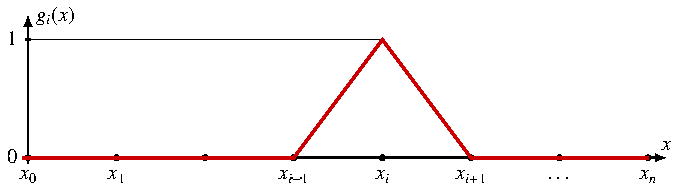
\includegraphics{chapters/090-pdenumerik/images/linear.pdf}
\caption{Die stückweise linearen Approximationsfunktionen $g_i(x)$
sind genau im Gitterpunkt $x_i$ von $0$ verschieden, wo der Wert $1$ ist,
und verschwinden in allen anderen Gitterpunkten.
\label{buch:pdenumerik:fem:fig:linear}}
\end{figure}
